\documentclass{standalone}
\usepackage{tikz}

\usetikzlibrary{calc}
\usetikzlibrary{shapes.geometric, arrows}

\tikzstyle{rect} = [
    rectangle,
    align=center,
    minimum width=3.1cm,
    minimum height=1cm,
    text centered,
    fill=color4!40,
    draw=color4dark,
    line width=1pt,
]
\tikzstyle{frect} = [rect, fill=color5!40, draw=color5dark]
\tikzstyle{brect} = [rect, fill=color1!40, draw=color1dark]
\tikzstyle{arrow} = [line width=1.2pt,->,>=stealth]
\tikzstyle{darrow} = [arrow, dashed]

\definecolor{color1}{HTML}{6bd2db}
\definecolor{color1dark}{HTML}{56a9b0}
\definecolor{color2}{HTML}{0ea7b5}
\definecolor{color3}{HTML}{0c457d}
\definecolor{color3dark}{HTML}{09325c}
\definecolor{color4}{HTML}{ffbe4f}
\definecolor{color4dark}{HTML}{cc993f}
\definecolor{color5}{HTML}{e8702a}
\definecolor{color5dark}{HTML}{ba5922}


\newcommand{\height}{2}
\newcommand{\width}{4}

\begin{document}
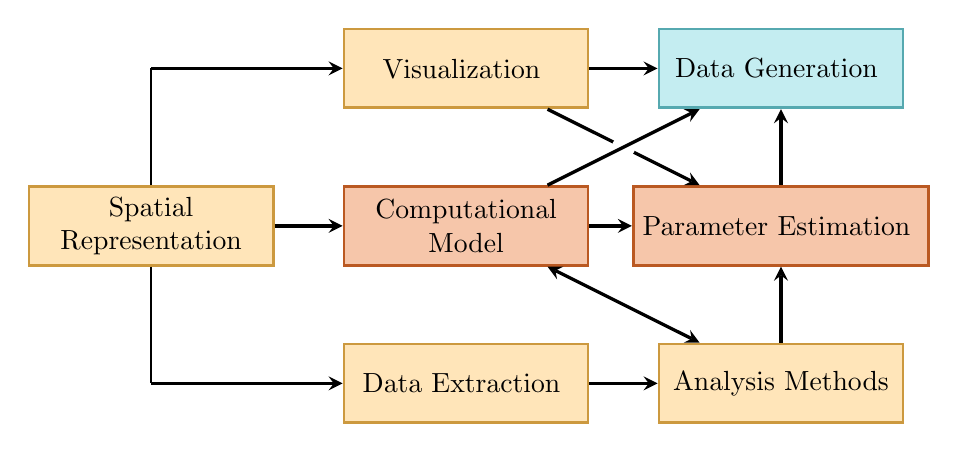
\begin{tikzpicture}[on top/.style={preaction={draw=white,-,line width=#1}},
on top/.default=4pt]
    \node (sr) [rect] at (-4, 0) {Spatial\\ Representation};%\\ $\{\vec{v}_i\}$};
    \node (mo) [frect] at (0,0) {Computational\\ Model};
    \node (vi) [rect] at (0,2) {
        Visualization
        %\includegraphics[width=1.5cm]
        %    {docs/source/_static/09395645494836445480/raw_pv/000000400.png}
        %\includegraphics[width=1.5cm]
        %    {docs/source/_static/09395645494836445480/masks/000000400.png}
    };
    \node (de) [rect] at (0,-2) {
        Data Extraction
        %\includegraphics[width=1.5cm]
        %    {docs/source/_static/fitting-methods/algorithm/interpolate-positions.png}
    };
    \node (pe) [frect] at (4,0) {
        Parameter Estimation
        % \includegraphics[width=1.5cm]
        %     {docs/source/_static/fitting-methods/progressions-4.png}
    };
    \node (am) [rect] at (4,-2) {Analysis Methods};

    \node (dg) [brect] at (4, 2) {
        Data Generation
        % \includegraphics[width=1.5cm]
        %     {docs/source/_static/09395645494836445480/images/000000400.png}
    };
    % \node (cs) [brect] at (8, 2.6) {Cell Segmentation};
    % \node (ct) [brect] at (8, 1.4) {Cell Tracking};

    % Draw arrows around corner
    \path [line width=1pt]
        (sr) edge (-4,2)
        (sr) edge (-4,-2);
    \path [arrow]
        (-4,2) edge (vi)
        (-4,-2) edge (de);
    \path [arrow]
        (sr) edge (mo)
        (de) edge (am)
        (vi) edge (dg)
        % (dg) edge (cs)
        % (dg) edge (ct)
        (vi) edge (pe)
        (am) edge (pe)
        (pe) edge (dg);
    \filldraw[fill=white,draw=white] ($1/2*(mo) + 1/2*(dg)$) circle (4pt);
    \path [arrow]
        (mo) edge (dg)
        (mo) edge (pe);
    \path [arrow,<->]
        (mo) edge (am);
\end{tikzpicture}
\end{document}
